\section{Mesh}

These routines describe and retreive the finite element mesh for this
computation.  A mesh, from the framework's perspective, is a list of
elements and nodes, together with uninterpreted data associated with each.
Elements map to nodes via the connectivity table for that element type.
Elements and nodes have both a global number (number in
the serial mesh) as well as a chunk-local number (number in the partitioned
mesh chunk).  The FEM framework currently uses the package Metis to do 
partitioning.

A simple program would set the serial mesh in init, get the partitioned
chunk in driver, and work on that chunk.  A more complex program would set
the initial mesh in init; then get, work on, update and repartition the mesh
several times in driver via \kw{FEM\_Update\_mesh}.

From \kw{init()}, the \kw{FEM\_Set\_} routines describe the serial mesh, which
will be partitioned into chunks.

From \kw{driver()}, the \kw{FEM\_Get\_} routines ask for the current mesh
chunk; the \kw{FEM\_Set\_} routines describe a new partitioned mesh chunk.  The
new chunk need not have the same number of elements or nodes as the old chunk;
but any new added nodes are assumed private (not shared).
\kw{FEM\_Update\_mesh} will reassemble a serial version of the mesh from the
new pieces and optionally repartition the serial mesh.



\prototype{FEM\_Get/Set\_elem}
\function{void FEM\_Set\_elem(int elType,int  nEl,int  doublePerEl,int  nodePerEl);}
\function{void FEM\_Get\_elem(int elType,int *nEl,int *doublePerEl,int *nodePerEl);}
\function{subroutine FEM\_Set\_elem(elType,nEl,doublePerEl,nodePerEl)}
  \args{integer, intent(in)  :: elType,nEl,doublePerEl,nodePerEl}
\function{subroutine FEM\_Get\_elem(elType,nEl,doublePerEl,nodePerEl)}
  \args{integer, intent(in)  :: elType}
  \args{integer, intent(out) :: nEl,doublePerEl,nodePerEl}

     Describe/retreive the number and type of elements.  \kw{ElType} is the
number of element types registered so far (the first element type is 1, then 2,
etc.).  \kw{nEl} is the number of elements being registered.  \kw{doublesPerEl}
and \kw{nodePerEl} are the number of doubles of user data, and nodes (respectively) associated with each element.
		
     \kw{doublePerEl} or \kw{nodePerEl} may be zero, indicating that no user
data or connectivity data (respectively) is associated with the element.

     You can make this and any other mesh setup calls in any order---there is no need 
to make them in linearly increasing order.  However, for a given type of element
\kw{FEM\_Set\_elem} must be called before setting that element's connectivity or data.


\prototype{FEM\_Get/Set\_elem\_conn}
\function{void FEM\_Set\_elem\_conn(int elType,const int *conn);}
\function{void FEM\_Get\_elem\_conn(int elType,int *conn);}
\function{subroutine FEM\_Set\_elem\_conn\_r(elType,conn)}
  \args{integer, intent(in)  :: elType}
  \args{integer, intent(in),  dimension(nodePerEl,nEl) :: conn}
\function{subroutine FEM\_Get\_elem\_conn\_r(elType,conn)}
  \args{integer, intent(in)  :: elType}
  \args{integer, intent(out), dimension(nodePerEl,nEl) :: conn}
\function{subroutine FEM\_Set\_elem\_conn\_c(elType,conn)}
  \args{integer, intent(in)  :: elType}
  \args{integer, intent(in),  dimension(nEl,nodePerEl) :: conn}
\function{subroutine FEM\_Get\_elem\_conn\_c(elType,conn)}
  \args{integer, intent(in)  :: elType}
  \args{integer, intent(out), dimension(nEl,nodePerEl) :: conn}

     Describe/retreive the element connectivity array for this element
     type.  The connectivity array is indexed by the element number,
     and gives the indices of the nodes surrounding the element.  It is
     hence \kw{nodePerEl*nEl} integers long.

     The C version array indices are zero-based, and must be stored in
     row-major order (a given element's surrounding nodes are stored
     contiguously in the conn array).  The Fortran version indices are
     one-based, and are available in row-major (named \_r) and
     column-major (named \_c) versions.  We recommend row-major storage
     because it results in better cache utilization (because the nodes
     around an element are stored contiguously).
     

\prototype{FEM\_Get/Set\_node}
\function{void FEM\_Set\_node(int  nNode,int  doublePerNode);}
\function{void FEM\_Get\_node(int *nNode,int *doublePerNode);}
\function{subroutine FEM\_Set\_node(nNode,doublePerNode)}
  \args{integer, intent(in)  :: nNode,doublePerNode}
\function{subroutine FEM\_Get\_node(nNode,doublePerNode)}
  \args{integer, intent(out) :: nNode,doublePerNode}

     Describe/retreive the number of nodes and doubles of user data
     associated with each node.  There is only one type of node, so no
     \kw{nodeType} identifier is needed.

     \kw{doublePerNode} may be zero, indicating that no user data is
     associated with each node.
     

\subsection{Mesh Data}
\prototype{FEM\_Get/Set\_data}
\function{void FEM\_Set\_node\_data(const double *data);}
\function{void FEM\_Get\_node\_data(double *data);}
\function{void FEM\_Set\_elem\_data(int elType,const double *data);}
\function{void FEM\_Get\_elem\_data(int elType,double *data);}
\function{subroutine FEM\_Set\_node\_data\_r(data)}
  \args{REAL*8, intent(in),  dimension(doublePerNode,nNode)  :: data}
\function{subroutine FEM\_Get\_node\_data\_r(data)}
  \args{REAL*8, intent(out), dimension(doublePerNode,nNode)  :: data}
\function{subroutine FEM\_Set\_node\_data\_c(data)}
  \args{REAL*8, intent(in),  dimension(nNode,doublePerNode)  :: data}
\function{subroutine FEM\_Get\_node\_data\_c(data)}
  \args{REAL*8, intent(out), dimension(nNode,doublePerNode)  :: data}

\function{subroutine FEM\_Set\_elem\_data\_r(elType,data)}
  \args{integer, intent(in)  :: elType}
  \args{REAL*8, intent(in),  dimension(doublePerElem,nElem)  :: data}
\function{subroutine FEM\_Get\_elem\_data\_r(elType,data)}
  \args{integer, intent(in)  :: elType}
  \args{REAL*8, intent(out), dimension(doublePerElem,nElem)  :: data}
\function{subroutine FEM\_Set\_elem\_data\_c(elType,data)}
  \args{integer, intent(in)  :: elType}
  \args{REAL*8, intent(in),  dimension(nElem,doublePerElem)  :: data}
\function{subroutine FEM\_Get\_elem\_data\_c(elType,data)}
  \args{integer, intent(in)  :: elType}
  \args{REAL*8, intent(out), dimension(nElem,doublePerElem)  :: data}

     Describe/retrieve the optional, uninterpreted user data associated with
each node and element.  This user data is partitioned and reassembled along
with the connectivity matrix, and may include initial conditions, node locations,
material types, or any other data needed or produced by the program.   The Fortran
arrays can be row- or column- major (see \kw{FEM\_Set\_elem\_conn} for
details).  The row-major form is preferred.


\subsection{Backward Compatability}
\prototype{FEM\_Set\_mesh}
\function{void FEM\_Set\_mesh(int nElem, int nNodes, int nodePerEl,const int* conn);}

     This is a convenience routine equivalent to:
\begin{alltt}
          FEM\_Set\_node(nNodes,0);
          FEM\_Set\_elem(0,nElem,0,nodePerEl);
          FEM\_Set\_elem\_Conn(0,conn);
\end{alltt}

\function{subroutine FEM\_Set\_mesh(nElem,nNodes,nodePerEl,conn)}
    \args{integer, intent(in) :: nElem, nNodes, nodePerEl}
    \args{integer, intent(in), dimension(nElem,nodePerEl) :: conn;}

     This is a convenience routine equivalent to:
\begin{alltt}
          CALL FEM\_Set\_node(nNodes,0)
          CALL FEM\_Set\_elem(1,nElem,0,nodePerEl)
          CALL FEM\_Set\_elem\_Conn\_c(1,conn)
\end{alltt}


\subsection{Sparse Data}

Sparse data is typically used to represent boundary conditions.  For
example, in a structural dynamics program typically some nodes have 
an imposed force or position.  The routines in this section are 
used to describe this kind of mesh-associated data---data that only 
applies to some ``sparse'' subset of the nodes or elements.  


\prototype{FEM\_Set\_sparse}
\function{void FEM\_Set\_sparse(int S\_id,int nRec,
         const int *nodes,int nodesPerRec,
         const void *data,int dataPerRec,int dataType);}
\function{subroutine FEM\_Set\_sparse(S\_id,nRec,nodes,nodesPerRec,data,dataPerRec,dataType)}
  \args{integer, intent(in) :: S\_id,nRec,nodesPerRec,dataPerRec,dataType}
  \args{integer, intent(in) :: nodes(nodesPerRec,nRec)}
  \args{varies,  intent(in) :: data(dataPerRec,nRec)}

Register \kw{nRec} sparse data records with the framework under the number \kw{S\_id}. 
The first call to \kw{FEM\_Set\_sparse} must give a \kw{S\_id} of zero in C (1 in fortran);
and subsequent calls to \kw{FEM\_Set\_sparse} must give increasing consecutive \kw{S\_id}s.

One sparse data record consists of some number of nodes, listed in the
\kw{nodes} array, and some amount of user data, listed in the data array.
Sparse data records are copied into the chunks that contains all that record's listed 
nodes.  Sparse data records are normally used to describe mesh boundary conditions--
for node-associated boundary conditions, \kw{nodesPerRec} is 1; for triangle-associated
boundary conditions, \kw{nodesPerRec} is 3.

In general, \kw{nodePerRec} gives the number of nodes associated with each
sparse data record, and \kw{nodes} gives the actual node numbers.
\kw{dataPerRec} gives the number of data items associated with each sparse 
data record, and \kw{dataType}, one of \kw{FEM\_BYTE}, \kw{FEM\_INT},
\kw{FEM\_REAL}, or \kw{FEM\_DOUBLE}, gives the type of each data item.
As usual, you may change or delete the \kw{nodes} and \kw{data} arrays after this
call returns.

For example, if the first set of sparse data is 17 sparse data records, each 
containing 2 nodes stored in \kw{bNodes} and 3 integers stored in \kw{bDesc}, 
we would make the call:
\begin{alltt}
/*C version*/
  FEM_Set_sparse(0,17, bNodes,2, bDesc,3,FEM_INT);
! Fortran version
  CALL FEM_Set_sparse(1,17, bNodes,2, bDesc,3,FEM_INT)
\end{alltt}

\prototype{FEM\_Set\_sparse\_elem}
\function{void FEM\_Set\_sparse\_elem(int S\_id,const int *rec2elem);}
\function{subroutine FEM\_Set\_sparse\_elem(S\_id,rec2elem)}
  \args{integer, intent(in) :: S\_id}
  \args{integer, intent(in) :: rec2elem(2,nRec)}

Attach the previously-set sparse records \kw{S\_id} to the given elements.
\kw{rec2elem} consists of pairs of integers---one for each sparse data record.
The first integer in the pair is the
element type to attach the sparse record to, and the second integer
gives the element number within that type.  For example, to attach
the 3 sparse records at \kw{S\_id} to the elements numbered 10, 11, and 12
of the element type \kw{elType}, use:

\begin{alltt}
/*C version*/
  int rec2elem[]={elType,10, elType,11, elType,12};
  FEM_Set_sparse_elem(S_id,rec2elem);
! Fortran version
  integer :: rec2elem(2,3);
  rec2elem(1,:)=elType
  rec2elem(2,1)=10; rec2elem(2,2)=11; rec2elem(2,3)=12;
  CALL FEM_Set_sparse_elem(S_id,rec2elem)
\end{alltt}


\prototype{FEM\_Get\_sparse}
\function{int  FEM\_Get\_sparse\_length(int S\_id);}
\function{void FEM\_Get\_sparse(int S\_id,int *nodes,void *data);}
\function{function FEM\_Get\_sparse\_length(S\_id);}
  \args{integer, intent(in) :: S\_id}
  \args{integer, intent(out) :: FEM\_Get\_sparse\_Length}
\function{subroutine FEM\_Get\_sparse(S\_id,nodes,data);}
  \args{integer, intent(in) :: S\_id}
  \args{integer, intent(out) :: nodes(nodesPerRec,FEM\_Get\_sparse\_Length(S\_id))}
  \args{varies,  intent(out) :: data(dataPerRec,FEM\_Get\_sparse\_Length(S\_id))}

Retrieve the previously registered sparse data from the framework.
\kw{FEM\_Get\_sparse\_length} returns the number of records of sparse
data registered under the given \kw{S\_id}; zero indicates no records
are available.  \kw{FEM\_Get\_sparse} returns you the actual nodes
(translated to local node numbers) and unchanged user data for
these sparse records.




%%%%%%%%%%%%%%%%%%%%%%%%%%%%%%%%%%%%%%%%%%%%%%%%%%%%%%%%%%%%%%%%%%%%%%%%%%%%%%%%%%%%%%%%
\newpage
\section{Mesh Modification}


\prototype{FEM\_Update\_mesh}
\function{void FEM\_Update\_mesh(FEM\_Update\_mesh\_fn routine, int callMeshUpdated,int doWhat);}
\function{subroutine FEM\_Update\_mesh(routine,callMeshUpdated,doWhat)}
    \args{external, intent(in) :: routine}
    \args{integer, intent(in) :: callMeshUpdated,doWhat}

Reassemble the mesh chunks from each partition into a single serial mesh,
and call the given \kw{routine} on the assembled mesh.
In this \kw{routine}, which runs on processor 0, the \kw{FEM\_Get} and \kw{FEM\_Set} routines
can manipulate the serial mesh.  The parameter \kw{callMeshUpdated}, which must
be non-zero, is passed down to \kw{routine} as \kw{routine(callMeshUpdated)}.

\kw{FEM\_Get} calls from
\kw{driver()} will only return the new mesh after a \kw{FEM\_Update\_mesh} call
where \kw{doWhat} is \kw{FEM\_MESH\_UPDATE}; otherwise \kw{FEM\_Get} from \kw{driver()} will still
return the old mesh.
\kw{FEM\_Update\_mesh} can only be called from driver; and must be called by the driver routine for
every chunk. 

%     If \kw{doRepartition} is 0, the mesh is not repartitioned, and \kw{FEM\_Update\_mesh}
%returns immediately.  If \kw{doRepartition} is 1, \kw{FEM\_Update\_mesh} blocks
%until the reassembled serial mesh is repartitioned back into chunks and redistributed.
%If \kw{doRepartition} is 2, 

\begin{center}
\begin{tabular}{|l|l|l|l|}\hline
\kw{doWhat} & Numeric & Repartition? & \kw{FEM\_Update\_mesh} \\\hline
\kw{FEM\_MESH\_OUTPUT} & 0 & No & \kw{driver()} continues alongside \kw{routine} \\
\kw{FEM\_MESH\_FINALIZE} & 2 & No & \kw{driver()} blocks until \kw{routine} finishes\\
\kw{FEM\_MESH\_UPDATE} & 1 & Yes & \kw{driver()} blocks for the new partition \\
\hline
\end{tabular}
\end{center}

For example, \kw{FEM\_Update\_mesh}(\uw{my\_output\_routine}, \uw{k}, \kw{FEM\_MESH\_OUTPUT}) 
reassembles the mesh and calls a routine named
\uw{my\_output\_routine(k)} while the driver routines continue with the computation.
This might be useful, for example, for writing out intermediate solutions as a 
single file; writing outputs from \kw{driver()} is more efficient but often results 
in a separate file for each mesh chunk.

   To block the driver routines during a call to a routine named
\uw{my\_finalize\_routine(k)}, such as 
at the end of the computation when the drivers have no other work to do, 
use \kw{FEM\_Update\_mesh}(\uw{my\_finalize\_routine}, \uw{k}, \kw{FEM\_MESH\_FINALIZE}).

     To reassemble, modify, and repartition the mesh, use
\kw{FEM\_Update\_mesh}(\uw{my\_update\_routine}, \uw{k}, \kw{FEM\_MESH\_UPDATE}).
It may be easier to perform major mesh modifications from \uw{my\_update\_routine(k)} than
the drivers, since the entire serial mesh is available to \uw{my\_update\_routine(k)}.

     \kw{FEM\_Update\_mesh} reassembles the serial mesh with an attempt to
     preserve the element and node global numbering.  If the new mesh
     has the same number and type of elements and nodes, the global
     numbers (and hence serial mesh) will be unchanged.  If new
     elements or nodes are added at each chunk, they will be assigned
     new unique global numbers.  If elements or nodes are removed,
     their global numbers are not re-used-- you can detect the
     resulting holes in the serial mesh since the user data associated
     with the deleted elements will be all zero.  Generally, however, it
     is less error-prone to perform mesh modifications only in \kw{driver()}
     or only in an update routine, rather than some in both.


%%%%%%%%%%%%%%%%%%%%%%%%%%%%%%%%%%%%%%%%%%%%%%%%%%%%%%%%%%%%%%%%%%%%%%%%%%%%%%%%%%%%%%%
\section {Mesh Ghosts}
An option to add ``ghosts'' to a mesh is provided by the framework. A ghost is a local read-only copy of a node or element that actually lives on another chunk.  Ghosts are typically added to the boundary of a chunk to allow the real (non-ghost) elements at the boundary to access values across the processor boundary.  This makes a chunk ``feel'' as if it was part of a complete unpartitioned mesh.


\begin{figure}[h]
\begin{center}
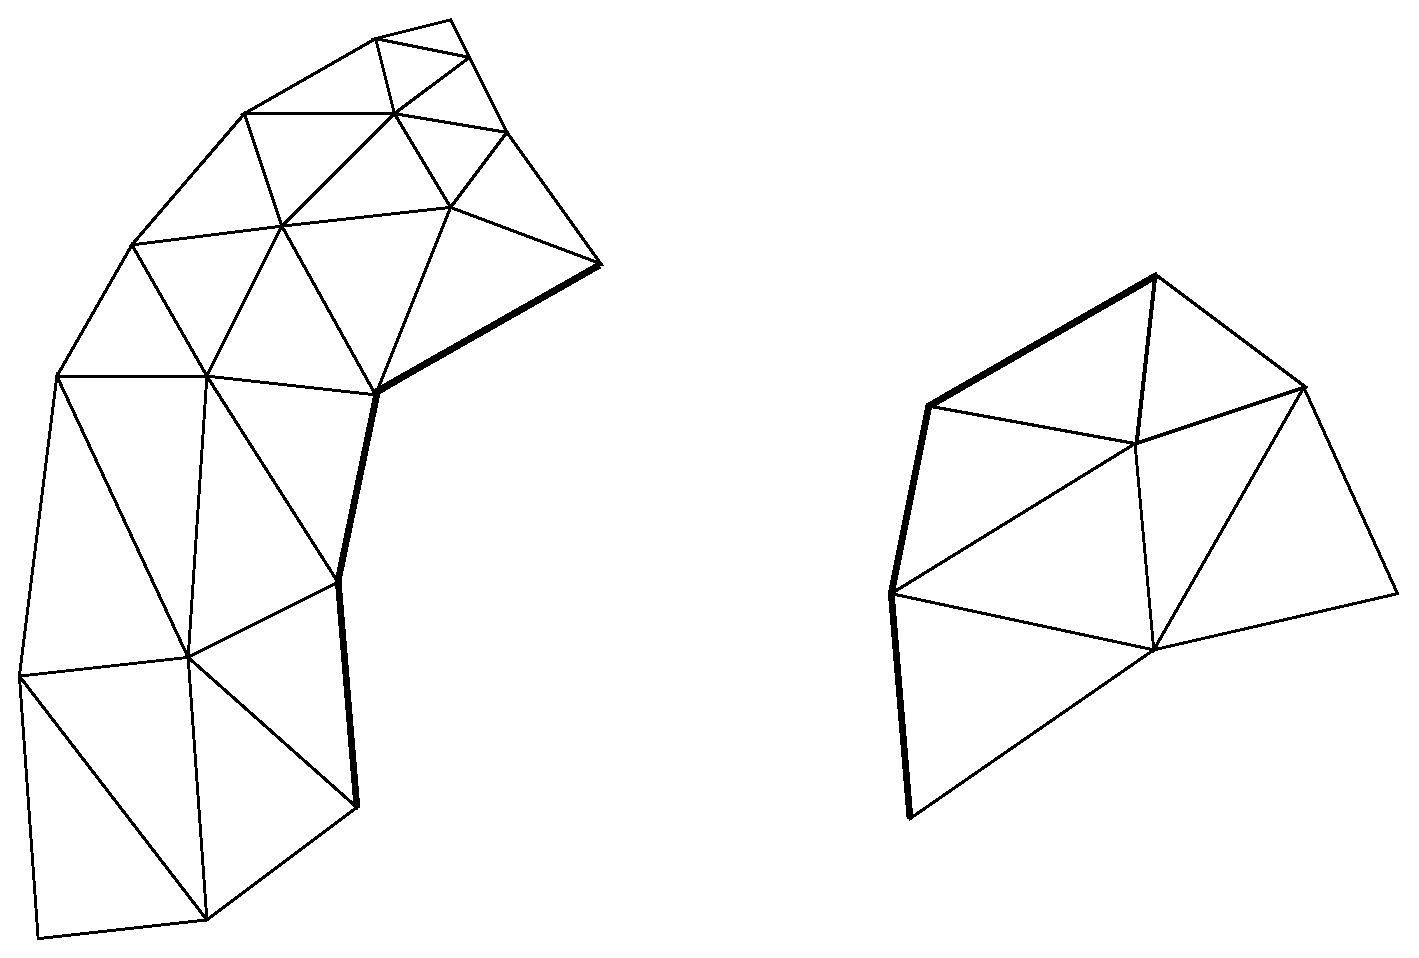
\includegraphics[width=2in]{fig/ghost_pre}
\end{center}
\caption{A small mesh partitioned into two pieces.}
\label{fig:ghostpre}
\end{figure}

In Figure~\ref{fig:ghostpre}, we begin with a small mesh partitioned
into pieces on the left and right.  In Figure~\ref{fig:ghostedge},
we have added ghost elements (dark hashing) that share an edge with
adjacent real elements (light hatching).  In Figure~\ref{fig:ghostnode},
we add ghost elements that share at least one node with adjacent 
real elements.

\begin{figure}[h]
\begin{center}
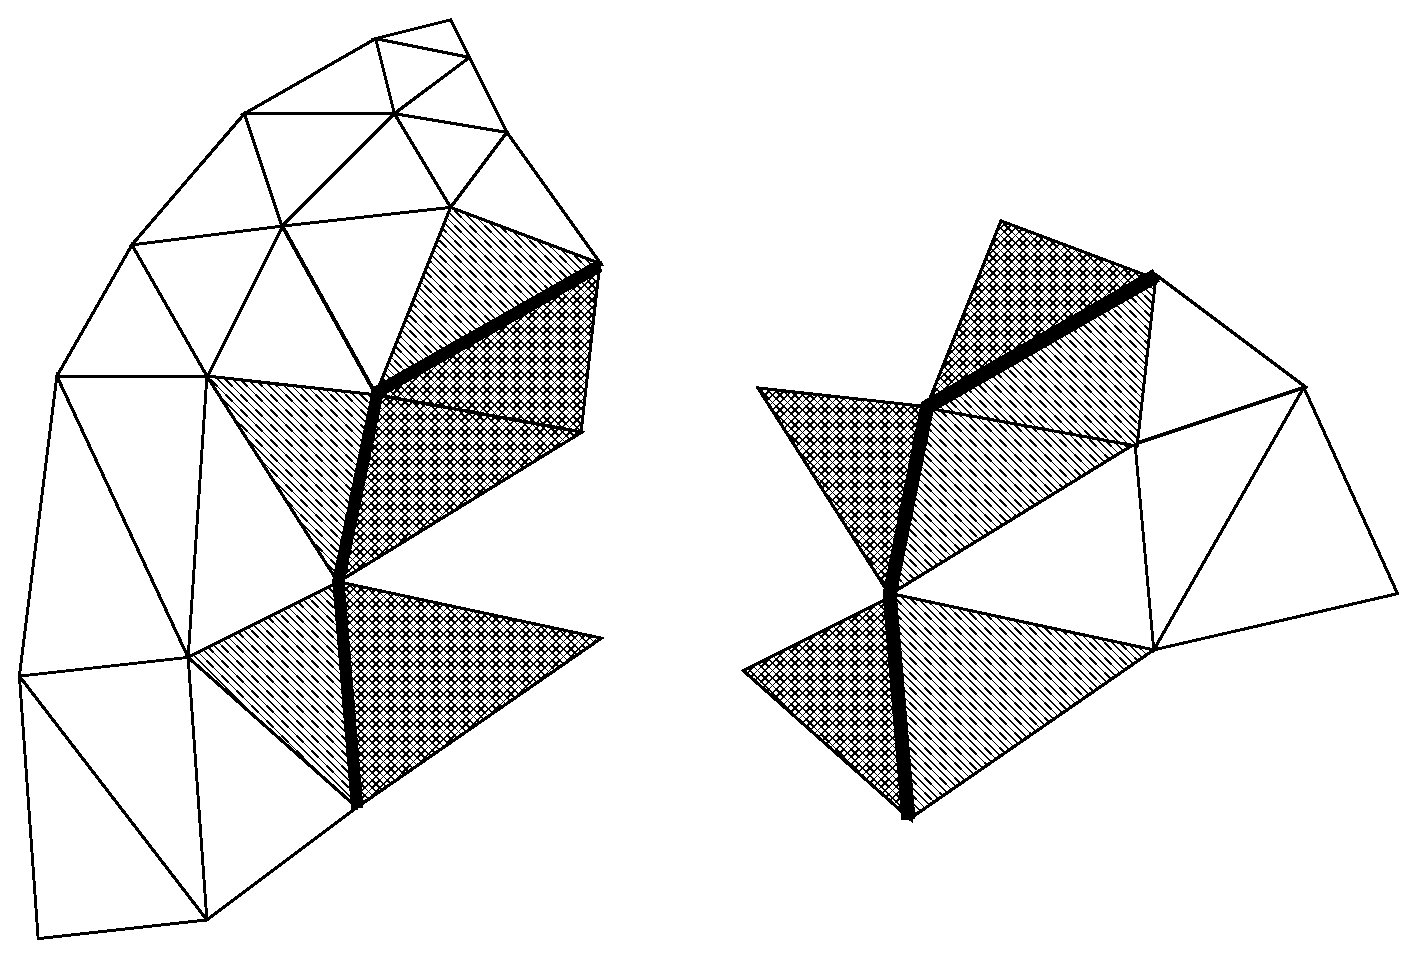
\includegraphics[width=2in]{fig/ghost_edge}
\end{center}
\caption{The same mesh with one layer of edge-adjacent ghosts.}
\label{fig:ghostedge}
\end{figure}

\begin{figure}[h]
\begin{center}
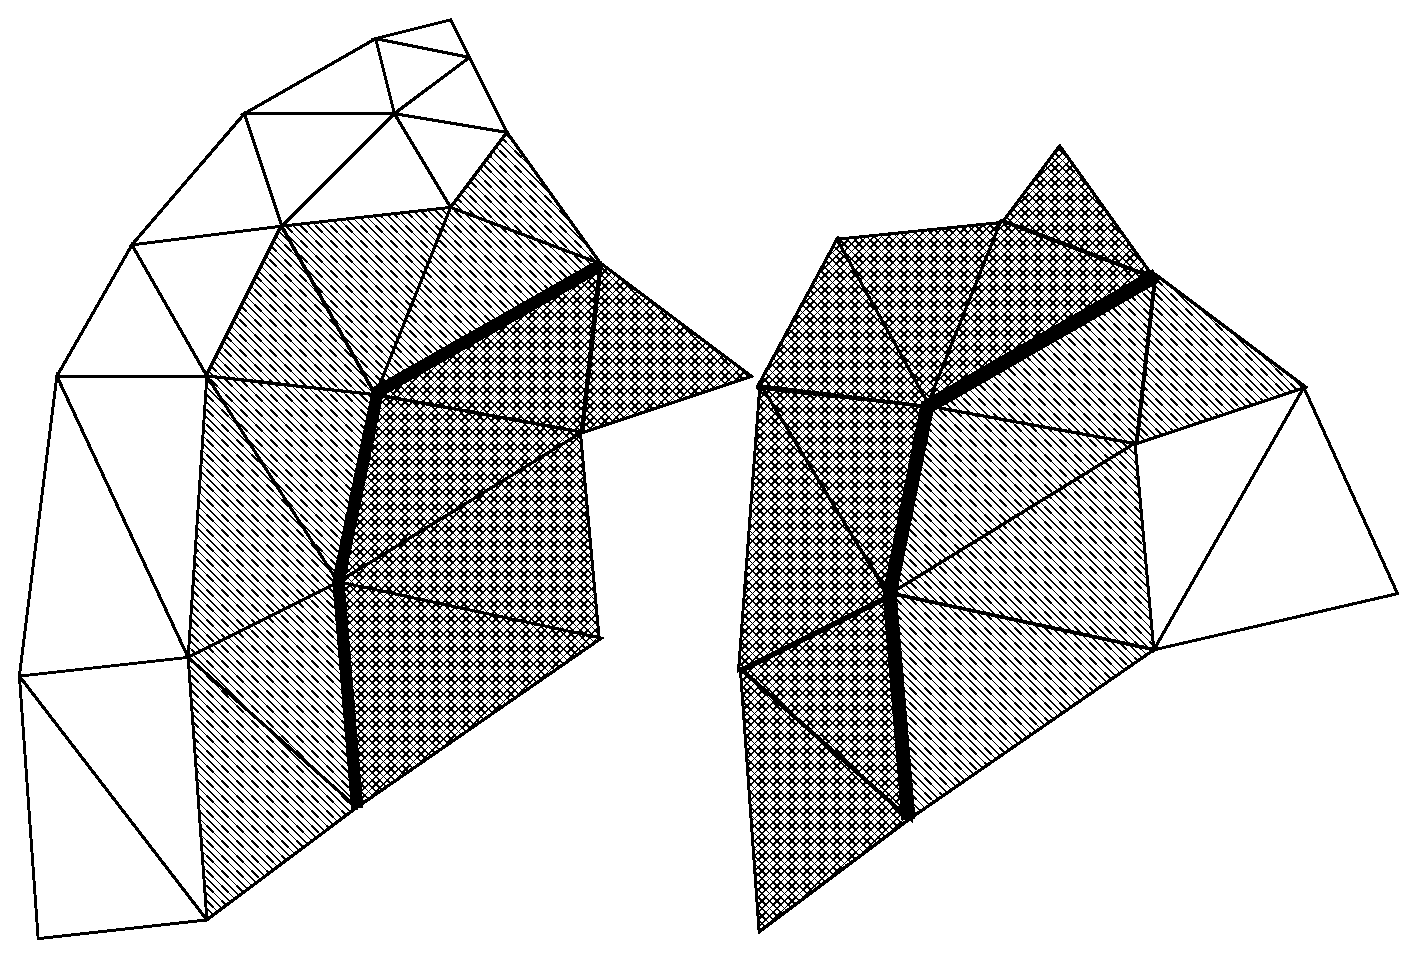
\includegraphics[width=2in]{fig/ghost_node}
\end{center}
\caption{The same mesh with one layer of node-adjacent ghosts.}
\label{fig:ghostnode}
\end{figure}



\subsection{Setting up the ghost layer}
The framework's ghost handling is element-centric. You specify which kinds of elements should be ghosts and how they connect by listing their ``tuples'' via calls in the \kw{init()} routine.  

\begin{itemize}
\item

\prototype{FEM\_Add\_ghost\_layer}
\function{void FEM\_Add\_ghost\_layer(int nodesPerTuple,int doAddNodes);}
\function{subroutine FEM\_Add\_ghost\_layer(nodesPerTuple,doAddNodes)}
  \args{integer, intent(in) :: nodesPerTuple,doAddNodes}
This routine creates a new layer of ghosts around each FEM chunk. \kw{nodesPerTuple} is the number of shared nodes that together form a ``tuple''. \kw{doAddNodes} specifies that you want ghost nodes as well as elements.

A tuple is an unordered set of nodes, and is an abstract way to describe which ghosts
your application needs---an element will be added to your chunk if it connects to at 
least one of your tuples.  For example, if you have a 3D, tetrahedral element that require ghosts 
on all 4 of its sides, this is equivalent to requiring ghosts of every element that shares all 3
nodes of one of your triangular faces, so for you a tuple is a 3-node face.  If you have a 2D shape
and want edge-adjacency, for you a tuple is a 2-node edge.  If you want node-adjacent ghosts,
a tuple is a single node.

Calling this routine several times creates several layers of ghost elements, and the different layers need not have the same parameters.

\item
\prototype{FEM\_Add\_ghost\_elem}
\function{void FEM\_Add\_ghost\_elem(int elType,int tuplesPerElem,const int *elem2tuple);}
\function{subroutine FEM\_Add\_ghost\_elem(elType,tuplesPerElem,elem2tuple)}
  \args{integer, intent(in) :: elType,tuplesPerElem}
  \args{integer, intent(in) :: elem2tuple(nodesPerTuple,tuplesPerElem)}

This call is used to specify which type of element is to be added to the current ghost layer. \kw{tuplesPerElem} and \kw{elem2tuple} specify a mapping between each element and the surrounding tuples.  The \kw{elem2tuple} table lists, for each tuple, the nodes of this element which form the tuple, specified as element-local numbers---indices into this element's connectivity entry. The \kw{elem2tuple} table should have nodesPerTuple*tuplesPerElem entries, and no entry should be greater than nodePerEl for that element type.

\kw{elem2tuple} can include special indices--- -1 for C, 0 for Fortran---that indicate the
corresponding tuple is shorter than usual.  For example, if \kw{nodesPerTuple} for this layer
is 4, for 4-node quadrilateral faces, you could set one entry in \kw{elem2tuple} to -1 to specify
a 3-node triangular face.  Tuples of different lengths will never match, so this is just
a simple way to add ghosts from two kinds of tuples at once.

\end{itemize}

The above two routines are always used together. For example, if your elements are 3-node triangles and you only require one shared node for inclusion in a single ghost layer, you would use:
\begin{alltt}
   FEM\_Add\_ghost\_layer(1,0); /* 1 node per tuple */
   const static int tri2node[]=\{0,1,2\};
   FEM\_Add\_ghost\_elem(0,3,tri2node); /* triangles are surrounded by 3 nodes */
\end{alltt}

If you require two shared nodes (a shared edge), the code will look like:
\begin{alltt}    
   FEM\_Add\_ghost\_layer(2,0); /* 2 nodes per tuple */
   const static int tri2edge[]=\{0,1,  1,2,  2,0\};
   FEM\_Add\_ghost\_elem(0,3,tri2edge); /*triangles are surrounded by 3 edges */
\end{alltt}



\subsection{Extracting the ghost layer}
After the ghost layer is created, we need a way to distinquish real nodes and elements 
from ghost nodes and elements. FEM\_Get\_node and FEM\_Get\_elem return the 
\textbf{total} number of nodes and elements, including ghosts. The routines below 
return the index of the first ghost node or element.

\prototype{FEM\_Get\_ghost}
\function{int FEM\_Get\_node\_ghost(void);}
\function{int FEM\_Get\_elem\_ghost(int elemType);}
The examples below iterate over the real and ghost elements.
\begin{alltt}
C version:
        int firstGhost,max;
        FEM\_Get\_node(\&max, \&ignored);
        firstGhost=FEM\_Get\_node\_ghost();
        for (i=0;i<firstGhost;i++)
                ... i is a real node...
        for (i=firstGhost;i<max;i++)
                ... i is a ghost node ...

Fortran version:
        call FEM\_Get\_node(max,ignored);
        firstGhost=FEM\_Get\_node\_ghost();
        do i=1,firstGhost-1
                ... i is a real node...
        end do
        do i=firstGhost,max
                ... i is a ghost node...
        end do
\end{alltt}

\subsection{Symmetries and Ghosts--Geometric Layer}

The FEM framework can create ghosts not only of things that are on other 
processors, but also for various problem symmetries, like mirror reflection,
and various types of periodicities.  The interface for these ghosts is 
simple---you ask for the symmetries to be created, then you will get 
extra ghosts along each symmetry boundary.  The symmetry ghosts are
updated properly during any communication, even if the symmetry ghosts
are ghosts of real local elements from the same chunk.


\begin{figure}[h]
\begin{center}
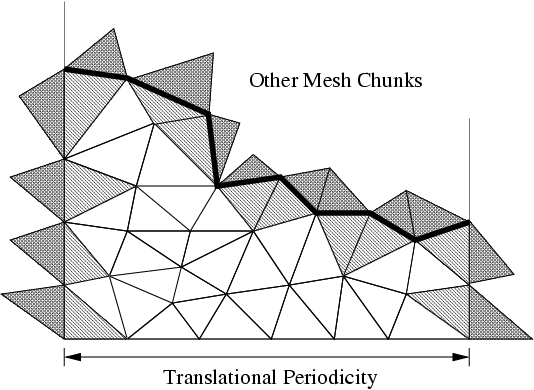
\includegraphics[width=3in]{fig/sym_ghost}
\end{center}
\caption{Illustrating symmetry ghost elements.}
\label{fig:symghost}
\end{figure}

Figure~\ref{fig:symghost} shows a chunk of a mesh for a 
rectangular domain with horizontal linear translational periodicity---that 
is, the domain repeats horizontally.
Symmetry ghosts lie along the left and right sides; ordinary cross-processor
parallel ghosts lie along the top edge where this chunk joins up with the
rest of the domain; and the external boundary along the bottom of the chunk
has no ghosts.



\prototype{FEM\_Add\_linear\_periodicity}
\function{void FEM\_Add\_linear\_periodicity(
        int nFaces,int nPer,
        const int *facesA,const int *facesB,
        int nNodes,const double *nodeLocs
        );}
\function{
SUBROUTINE FEM\_Add\_linear\_periodicity(nFaces,nPer,facesA,facesB,
                                nNodes,nodeLocs)}
  \args{integer, intent(in) :: nFaces, nPer, nNodes}
  \args{integer, intent(in) :: facesA(nPer,nFaces), facesB(nPer,nFaces)}
  \args{double precision, intent(in) :: nodeLocs(3,nNodes)}

Make facesA and facesB match up under linear translation.
Each face of facesA must match up with exactly one face of
facesB, but both the faces and the nodes within a face can be
permuted in any order---the order is recovered by matching 3d locations
in the nodeLocs array.

This call can be repeated, for example if the domain is periodic along several
directions.  This call can only be issued from \kw{init()}.



\prototype{FEM\_Sym\_coordinates}
\function{void FEM\_Sym\_coordinates(int elTypeOrMinusOne,double *locs);}
\function{SUBROUTINE FEM\_Sym\_coordinates(elTypeOrZero,locs)}
  \args{integer, intent(in) :: elTypeOrZero}
  \args{double precision, intent(inout) :: locs(3,<number of items>)}

This call adjusts the 3d locations listed in \kw{locs} so they respect the symmetries
of their corresponding item.  If elTypeOrZero is an element type,
the locations are adjusted to match with the corresponding element;
if elTypeOrZero is zero, the locations are adjusted to match up with
the corresponding node.

This call is needed because symmetry ghost nodes and elements
initially have their original locations, which must be adjusted
to respect the symmetry boundaries.  Thus this call is needed
both for initial location data (e.g., from \kw{FEM\_Get\_node\_data})
as well as any communicated location data (e.g., from
\kw{FEM\_Update\_ghost\_field}).

This call can only be issued from \kw{driver()}.



\subsection{Symmetries and Ghosts--Lower Layer}

The geometric symmetry layer in the preceeding section is actually
a thin wrapper around this lower, more difficult to use layer.

\prototype{FEM\_Set\_sym\_nodes}
\function{void FEM\_Set\_sym\_nodes(const int *canon,const int *sym);}
\function{SUBROUTINE FEM\_Set\_sym\_nodes(canon,sym)}
  \args{integer, intent(in) :: canon(nNodes)}
  \args{integer, intent(in) :: sym(nNodes)}

This call describes all possible symmetries in an extremely terse format.
It can only be called from \kw{init()}.
The ``canonicalization array'' canon maps nodes to their canonical 
representative---if canon($i$)=canon($j$), nodes $i$ and $j$ are 
images of each other under some symmetry.  The sym array has bits set
for each symmetry boundary passing through a node.

For example, a 2d domain with 6 elements A, B, C, D, E, and F and 12 
nodes numbered 1-12 that is 
mirror-symmetric on the horizontal boundaries but periodic in the 
vertical boundaries would look like:

\begin{alltt}
   D^'|  D^ |  E^ |  F^ |  F^`
   -  1  -  2  -  3  -  4  -
   A' |  A  |  B  |  C  |  C`
   -  5  -  6  -  7  -  8  -
   D' |  D  |  E  |  F  |  F`
   -  9  - 10  -  11 -  12 -
   Av'|  Av |  Bv |  Cv |  Cv`

  v indicates the value has been shifted down (bottom boundary),
  ^ indicates the value has been shifted up (top boundary),
  ' indicates the value has been copied from the left (right boundary),
  ` indicates the value has been copied from the right (left boundary).
\end{alltt}

If we mark the left border with 1, the top with 2, the right with 4,
and the bottom with 8, this situation is indicated by topologically pasting the 
top row to the bottom row by setting their \kw{canon} entries equal, and 
marking each node with its symmetries.

\begin{center}
\begin{tabular}{|l|l|l|}\hline
  Node & \kw{canon} &  \kw{sym}              \\\hline
    1  &    1  &      3 (left + top)   \\
    2  &    2  &      2 (top)   \\
    3  &    3  &      2 (top)   \\
    4  &    4  &      6 (top + right)   \\
    5  &    5  &      1 (left)   \\
    6  &    6  &      0 (none)   \\
    7  &    7  &      0 (none)   \\
    8  &    8  &      4 (right)   \\
    9  &    1  &      9 (left+bottom)    \\
    10 &    2  &      8 (bottom)   \\
    11 &    3  &      8 (bottom)   \\
    12 &    4  &      12 (bottom+right)   \\
\hline
\end{tabular}
\end{center}


\prototype{FEM\_Get\_sym}
\function{void FEM\_Get\_sym(int elTypeOrMinusOne,int *destSym);}
\function{void FEM\_Get\_sym(elTypeOrZero,destSym);}
  \args{integer, intent(in) :: elTypeOrMinusOne }
  \args{integer, intent(out) :: destSym(nItems)}

This call extracts the list of symmetry conditions that apply to 
an item type.  If elType is an element type, it returns the
symmetry conditions that apply to that element type; if elType is
-1 (zero for Fortran), it returns the symmetry conditions that apply
to the nodes.  Symmetry conditions are normally only nonzero
for ghost nodes and elements.


Mirror symmetry conditions are not yet supported, nor are
multiple layers of symmetry ghosts.  

% FIXME: document these
% void FEM_Set_partition(int *elem2chunk)
% int FTN_NAME(FEM_GET_COMM_PARTNERS,fem_get_comm_partners)(void)
% int FTN_NAME(FEM_GET_COMM_PARTNER,fem_get_comm_partner)(int *partnerNo)
% int FTN_NAME(FEM_GET_COMM_COUNT,fem_get_comm_count)(int *partnerNo)
% void FTN_NAME(FEM_GET_COMM_NODES,fem_get_comm_nodes)(int *pNo,int *nodeNos)
% void FTN_NAME(FEM_GET_ELEM_NUMBERS,fem_get_elem_numbers)(int *gNo)
% void fem_get_node_numbers(int *gNo)
